%----------------------------------------------------------------------------------------
%
% A LaTeX-template for 1DV510. Modified and translated by Björn Lindenberg at LNU.
% Based on an original master thesis template created by Marcus Wilhelmsson at LNU.
%
%----------------------------------------------------------------------------------------

% Settings and document configuration

\documentclass[a4paper,12pt]{article} 
\usepackage[T1]{fontenc} 
\usepackage{times} 
\usepackage[swedish,english]{babel} 
\usepackage[utf8]{inputenc} 
\usepackage{dtk-logos} 
\usepackage{wallpaper} 
\usepackage[absolute]{textpos} 
\usepackage[top=2cm, bottom=2.5cm, left=3cm, right=3cm]{geometry} 
\usepackage[parfill]{parskip} 
\usepackage{csquotes} 
\usepackage{float} 
\usepackage{lipsum} % Used for dummy text. Can be removed.
\usepackage{listings, color}

\lstdefinestyle{Asm}{
  belowcaptionskip=1\baselineskip,
  breaklines=true,
  frame=L,
  xleftmargin=\parindent,
  language=[x86masm]Assembler,
  showstringspaces=false,
  basicstyle=\footnotesize\ttfamily,
  keywordstyle=\bfseries\color{purple!40!black},
  commentstyle=\itshape\color{green!40!black},
  identifierstyle=\color{blue},
  stringstyle=\color{orange},
}

% Fontsizes for section headings.
\usepackage{sectsty} 
\sectionfont{\fontsize{14}{15}\selectfont}
\subsectionfont{\fontsize{12}{15}\selectfont}
\subsubsectionfont{\fontsize{12}{15}\selectfont}

%----------------------------------------------------------------------------------------
%	This part is used for the text box on the title page
%----------------------------------------------------------------------------------------
\newsavebox{\mybox}
\newlength{\mydepth}
\newlength{\myheight}

\newenvironment{sidebar}%
{\begin{lrbox}{\mybox}\begin{minipage}{\textwidth}}%
{\end{minipage}\end{lrbox}%
 \settodepth{\mydepth}{\usebox{\mybox}}%
 \settoheight{\myheight}{\usebox{\mybox}}%
 \addtolength{\myheight}{\mydepth}%
 \noindent\makebox[0pt]{\hspace{-20pt}\rule[-\mydepth]{1pt}{\myheight}}%
 \usebox{\mybox}}

%----------------------------------------------------------------------------------------
%	Title
%----------------------------------------------------------------------------------------
\newcommand\BackgroundPic{
    \put(-2,-3){
    
\includegraphics[keepaspectratio,scale=0.3]{img/lnu_etch.png} % Background image
    }
}
\newcommand\BackgroundPicLogo{
    \put(30,740){
    
\includegraphics[keepaspectratio,scale=0.10]{img/logo.png} % LNU logo
    }
}

\title{
\vspace{-8cm}
\begin{sidebar}
    \vspace{10cm}
    \normalfont \normalsize
    \huge Computer Technology I\\ % Main title
    \vspace{-1.3cm}
\end{sidebar}
\vspace{3cm}
\begin{flushleft}
    \huge Lab. 3 : Interrupts % Subtitle
     \small \\ \emph{}
\end{flushleft}
\null
\vfill
\begin{textblock}{5}(10,13)
\begin{flushright}
\begin{minipage}{\textwidth}
\begin{flushleft} \large
\emph{Author:}\textsc{ Loic GALLAND, Leonardo PEDRO}\\  % Author
\emph{Supervisor:}  \textsc{} \\  % Author
\emph{Semester:} Autumn 2019\\ % Semester
\emph{Area:} Computer Science \\ % Area
\emph{Course code:} 1DT301 % Course
\end{flushleft}
\end{minipage}
\end{flushright}
\end{textblock}
}

\date{} % Empty date command. Use \today inside for today's date.
\author{} % Normally one would use this to define authors. However in this case the title command takes care of everything, so we leave the field empty to get rid of warnings. 

\begin{document}

\pagenumbering{gobble} % Turn off page numbering
\newgeometry{left=5cm}
\AddToShipoutPicture*{\BackgroundPic} % Adds the background image to the title page
\AddToShipoutPicture*{\BackgroundPicLogo} % Adds the logo to the title page
\maketitle % Prints the title
\restoregeometry
\clearpage

\pagenumbering{roman} % Roman page numbering for abstract page


\selectlanguage{english}

\newpage

\pagenumbering{gobble} % Turn off page numbering
\tableofcontents 

\newpage
\pagenumbering{arabic} % Turn on page numbering


\section{Task 1 - }

\textit{Write a program that turns ON and OFF a LED with a push button. The LED will be extinguished
when pressing the button.
The program will use Interrupt. Connect the push buttons to PORT D.
The program should have a main program that runs in a loop and wait for the interrupts. An
interrupt routine is called when the push button is pressed. Each time the button is pressed, the
lamp should switch from ‘OFF’ to ‘ON’, or from ‘ON’ to ‘OFF’.}

\lstset{style=Asm}
\begin{lstlisting}
;>>>>>>>>>>>>>>>>>>>>>>>>>>>>>>>>>>>>>>>>>>>>>>>>>>>>>>>>>>>
; 1DT301, Computer Technology I
; Date: 2019-09-29
; Author:
; Loic GALLAND
; Leonardo PEDRO
;
; Lab number: 3
; Title: How to use interrupts
;
; Hardware: STK600, CPU ATmega2560
;
; Function: Program that when clicking on a switch the LEDs switch from ON to OFF and vice versa. It is using interupts to do it.
;
; Input ports: PORTD
;
; Output ports: PORTB
;
; Subroutines: If applicable.
; Included files: m2560def.inc
;<<<<<<<<<<<<<<<<<<<<<<<<<<<<<<<<<<<<<<<<<<<<<<<<<<<<<<<<<<<
.include "m2560def.inc"

.org 0x00	;Location where the program will start
rjmp start

.org INT0addr	;INT0 interrupt address
rjmp interrupt_0

.org 0x72

start:
.def LIGHT = r21	;Give a name to r21
; Initialize SP, Stack Pointer
ldi r20, HIGH(RAMEND) ; R20 = high part of RAMEND address
out SPH,R20 ; SPH = high part of RAMEND address
ldi R20, low(RAMEND) ; R20 = low part of RAMEND address
out SPL,R20 ; SPL = low part of RAMEND address

ldi r16,0xFF	;Load 0xFF into r16 to initialize PORTB
out DDRB,r16	
ldi r16,0x00	;Load 0x00 into r16 and initialize PORTD
out DDRD,r16

ldi r18, 0xFF	;initiliaze the LEDs (turn them off)
out PORTB, r18

mov LIGHT,r18	;Copy the r18 into "LIGHT"
;Initialised the Interrupts
ldi r16, 0b00000010	;INT0 falling edge
sts EICRA, r16	;Setup internal 

ldi r16, 0b00000001	;INT0 enable, pin 0 of PORT D
out EIMSK, r16
sei	;Global interrupt enable

main:
	out PORTB, LIGHT	;Turn on the LEDs
rjmp main

interrupt_0:
	com LIGHT	;Change the 0s into 1s, to show the lights on
RETI	
\end{lstlisting}
This is the flowchart of the task 1:
\begin{center}
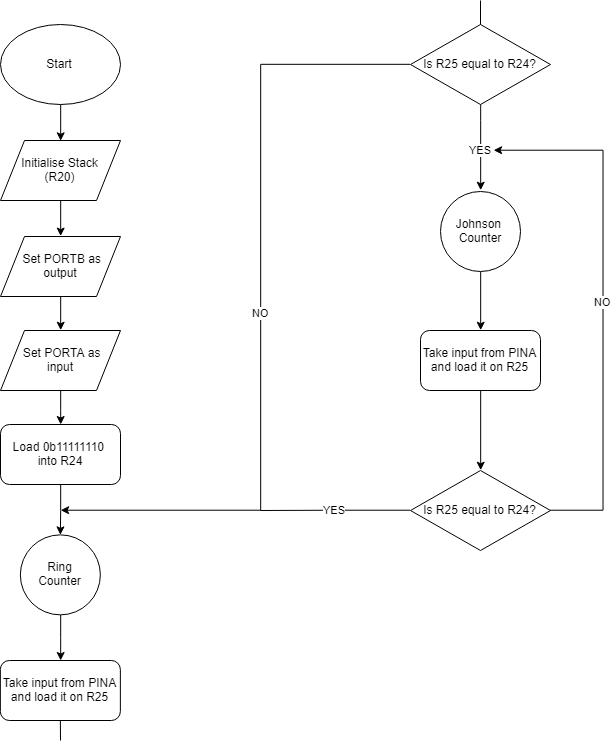
\includegraphics[scale=0.7]{img/Task1.png}
\end{center}
\newpage
\section{Task 2 - Switch – Ringcounter / Johnsoncounter, with interrupt}
\textit{Write a program that by means of a switch can choose to flash 8 LEDs either in the form of a ring
counter or in the form of a Johnson counter. Use the switch SW0 connected to PORTD to switch
between the two counters. Each time the button is pressed, a shift between the two counters
should take place. By using interrupts you’ll swap directly with no delay.}

\lstset{style=Asm}
\begin{lstlisting}
;>>>>>>>>>>>>>>>>>>>>>>>>>>>>>>>>>>>>>>>>>>>>>>>>>>>>>>>>>>>
; 1DT301, Computer Technology I
; Date: 2019-09-29
; Author:
; Loic GALLAND
; Leonardo PEDRO
;
; Lab number: 3
; Title: How to use interrupts
;
; Hardware: STK600, CPU ATmega2560
;
; Function: Program that when clicking on a switch switches between Ring Counter and Johnson Counter
;
; Input ports: PORTD
;
; Output ports: PORTB
;
; Subroutines: If applicable.
; Included files: m2560def.inc
;<<<<<<<<<<<<<<<<<<<<<<<<<<<<<<<<<<<<<<<<<<<<<<<<<<<<<<<<<<<
.include "m2560def.inc"

.org 0x00
rjmp start

.org INT0addr	;Address of the Interrupt 0
rjmp interrupt

.org 0x72

start:
; Initialize SP, Stack Pointer
ldi r20, HIGH(RAMEND) ; R20 = high part of RAMEND address
out SPH,R20 ; SPH = high part of RAMEND address
ldi R20, low(RAMEND) ; R20 = low part of RAMEND address
out SPL,R20 ; SPL = low part of RAMEND address

ldi r20,0b00000010 ;Setting INT0 into falling edge
sts EICRA,r20
ldi r20,0b00000001 ;INT0 enable, pin 0 of Port D
out EIMSK,r20

ldi r17,0xFF	;Set PORTB as output
out DDRB, r17

ldi r17,0x00	;Set PORTD as input
out DDRD,r17

.equ Counter = 0xFF	;This variable will help us to know in which counter the program is to switch to the other one 
.equ DOWN = 0	;Variable to check if the Johnson counter is going left or right 
.def LED = r22	;Giving a name to r22 like if it a variable
.def Status = r23	;Same here
ldi Status,DOWN	;Loading 0 (DOWN) into R23(Status)

ldi r16, Counter	;iniatialize LEDs (Turn them off)
out PORTB,r16

call reset ;To reset the LEDs 
sei	;Global interrupt enable

main:
	cpi r16, Counter	;Check in which program it is
		breq Ring_Johnson	;Send to Johnson counter if r16 = 0xFF

	Johnson_Ring:	;Else goes here ans send to Ring counter
		
		call RC	;Call the Ring Counter routine
	rjmp main

	Ring_Johnson:
		call JC	;Call the Johnson Counter routine

rjmp main

reset:	;To reset the LEDS
ldi LED,0b11111110	;Load 254 into LED.
out PORTB,LED	;Show the result on the LEDs.
RET	;Return to where the reset was called.

RC:	;RING COUNTER
	SBIS PORTB,PINB7 ;If the LED7 is ON then reset the LEDs otherwise skip the next line.
		ldi LED,0b11111110
	SBIC PORTB,PINB7	;If the LED7 is OFF then Rotate otherwise skip the next line 
		rol LED	;Rotate to the left 
	out PORTB,LED	;output to PORTB to show the LEDs
	call Delay	;Delay of 0.5 sec
rjmp main

JC:	;JOHNSON COUNTER
	cpi Status,DOWN	;Check if the LEDs needs to go left
		breq JCLEFT	;IF Status =0x00 go to JCLEFT
	rjmp JCRIGHT	;Otherwise go to JCRIGHT
	
	shift_left_right:
	ldi LED, 0b10000000	;Reset the LEDs to make go right
	out PORTB,LED
	call Delay
	com Status	;Change the status to 0xFF
	rjmp JCRIGHT

	shift_right_left:
	com Status	;Change the status to 0x00
	rjmp JCLEFT	;Jump back to JCLEFT

	JCLEFT:
		sbis PORTB,PINB7	;Checks if LED7 is on
			rjmp shift_left_right	;if it is on then jump to shift_left_right
		LSL LED ;Otherwise Logical shift to the left for the LEDs
		out PORTB, LED	;output to PORTB 
		CALL Delay	;Delay of 0.5 sec 
	rjmp finish
		
	JCRIGHT:
		sbic PORTB,PINB0	;If LED7 is off then jump to shift_right_left
			rjmp shift_right_left
		ASR LED	;Otherwise skip the jump and Arithmetic shift right
		out PORTB,LED
		CALL Delay

finish:
RET	;Return to where to it was called

interrupt:
com r16	;To change between 
call reset
RETI

Delay:
; Generated by delay loop calculator
; at http://www.bretmulvey.com/avrdelay.html
; Delay 500 000 cycles
; 500ms at 1 MHz
    ldi  r18, 3
    ldi  r19, 138
    ldi  r20, 86
L1: dec  r20
    brne L1
    dec  r19
    brne L1
    dec  r18
    brne L1
    rjmp PC+1
RET
\end{lstlisting}
\newpage
This is the flowchart of the task 2:
\begin{center}
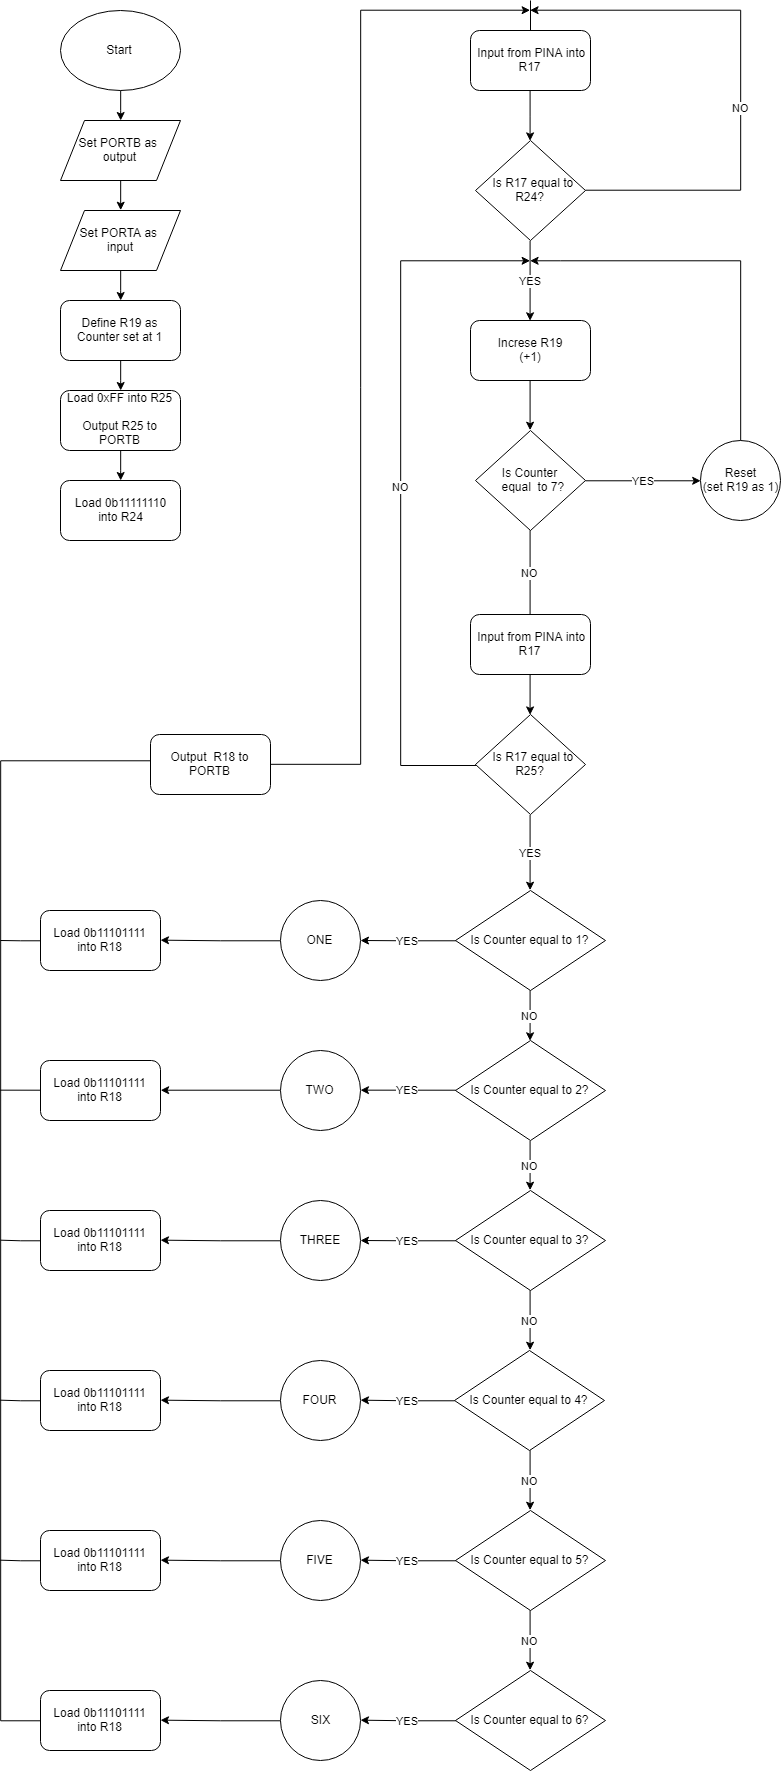
\includegraphics[scale=0.6]{img/Task2.png}
\end{center}

\newpage
\section{Task 3 - Rear lights on a car}
\textit{Program that simulates the rear lights on a car
The 8 LEDs should behave like the rear lights.}

\lstset{style=Asm}
\begin{lstlisting}
;>>>>>>>>>>>>>>>>>>>>>>>>>>>>>>>>>>>>>>>>>>>>>>>>>>>>>>>>>>>
; 1DT301, Computer Technology I
; Date: 2019-09-29
; Author:
; Loic GALLAND
; Leonardo PEDRO
;
; Lab number: 3
; Title: How to use interrupts
;
; Hardware: STK600, CPU ATmega2560
;
; Function: Program that acts like the rear lights of a car. Either blinking right, left or just normal
;
; Input ports: PORTD
;
; Output ports: PORTB
;
; Subroutines: If applicable.
; Included files: m2560def.inc
;<<<<<<<<<<<<<<<<<<<<<<<<<<<<<<<<<<<<<<<<<<<<<<<<<<<<<<<<<<<
.include "m2560def.inc"

.org 0x00
rjmp start

.org INT0addr	;Address of Interrupt 0
rjmp BlinkRight	

.org INT1addr  ;Address of Interrupt 1
rjmp normal

.org INT2addr	;Address of Interrupt 2
rjmp BlinkLeft

.org 0x72

start:
; Initialize SP, Stack Pointer
ldi r20, HIGH(RAMEND) ; R20 = high part of RAMEND address
out SPH,R20 ; SPH = high part of RAMEND address
ldi R20, low(RAMEND) ; R20 = low part of RAMEND address
out SPL,R20 ; SPL = low part of RAMEND address

ldi r20,0b00101010 ;Setting INT0-INT1-INT2 into falling edge
sts EICRA,r20
ldi r20,0b00000111 ;Enable INT0-INT1-INT2
out EIMSK,r20

ldi r17,0xFF	;Set PORTB as output
out DDRB, r17

ldi r17,0x00	;Set PORTD as input
out DDRD,r17

ldi r16, 0xFF	;Initialized LED state
out PORTB, r16

.def LED = r16	;Give the name "LED" to the register number 16
.def Normal_Right = r22	;Give the name "Normal_Right" to the register number 22, will be used to simulate the left rear light
ldi Normal_Right, 0b11000000
.def Normal_Left = r21	;Give the name "Normal_Left" to the register number 21 will be used to simulate the right rear light
ldi Normal_Left,0b00000011
sei	;Global interrupt enable


ldi r23, 1	;Variable to know in which configuration we are in.


Main:
	cpi r23, 1	;If r23 = 1 then branch to NLED which is the normal LEDs:
	breq NLED			

	cpi r23, 2	;If r23 = 2 then branch to BLeft which is the blinking to left.
	breq BLeft

	cpi r23, 3 ;If r23 = 3 then branch to BLeft which is the blinking to left.
	breq BRight


rjmp Main

NLED:	;Routine for turning on the both rear lights, for the "normal" configuration
ldi LED, 0b00111100
out PORTB, LED
rjmp Main	;Jumps back to "Main" loop 

BLeft: ;RING COUNTER

	SBIS PORTB,PINB7 ;If the LED7 is on then reset the LEDs otherwise skip the next line
		ldi LED,0b00010000
	SBIC PORTB,PINB7	;If the LED7 is not on then Rotate otherwise skip the next line 
		rol LED	;Rotate to the left 
	mov r17,LED	;Copy the info of "LED" and load it into r17
	add r17,Normal_Left	;Add the 0b00000011 to r17 to make it become like that: 00010011 for the first round 
	COM r17	;One's Complement of r17 to switch the 0s into 1s to output the correct binary code for the LEDs
	out PORTB,r17	;output to PORTB to show the LEDs
	call Delay	;Delay of 0.5 sec
rjmp main


BRight:
	SBIS PORTB,PINB0 ;If the LED0 is on then reset the LEDs otherwise skip the next line
		ldi LED,0b00001000
	SBIC PORTB,PINB0	;If the LED0 is not on then Rotate otherwise skip the next line 
		ror LED	;Rotate to the left 
	mov r17,LED	;Copy the info of "LED" and load it into r17
	add r17,Normal_Right	;Add the 0b00000011 to r17 to make it become like that: 00010011 for the first round 
	COM r17	;One's Complement of r17 to switch the 0s into 1s to output the correct binary code for the LEDs
	out PORTB,R17	;output to PORTB to show the LEDs
	call Delay	;Delay of 0.5 sec
rjmp main


normal:	;Interupt for the normal lights
ldi r23, 1	;Load 1 into r23 to know later on which program we are in
RETI	;Return to where the interrupt interrupted the code 

BlinkLeft:	;Interrupt for when we need to blink left 
ldi r23, 2	;Load 2 into r23 to know later on which program we are in
ldi LED,0b00010000	;Initial state of the LEDs 
RETI	;Return to where the interrupt interrupted the code 

BlinkRight:	;Interrupt for when we need to blink left 
ldi r23, 3	;Load 3 into r23 to know later on which program we are in
ldi LED,0b00001000	;Initial state of the LEDs
RETI	;Return to where the interrupt interrupted the code 

Delay:
; Generated by delay loop calculator
; at http://www.bretmulvey.com/avrdelay.html
; Delay 500 000 cycles
; 500ms at 1 MHz
    ldi  r18, 3
    ldi  r19, 138
    ldi  r20, 86
L1: dec  r20
    brne L1
    dec  r19
    brne L1
    dec  r18
    brne L1
    rjmp PC+1
RET
\end{lstlisting}

\newpage
This is the flowchart of the task 3:
\begin{center}
%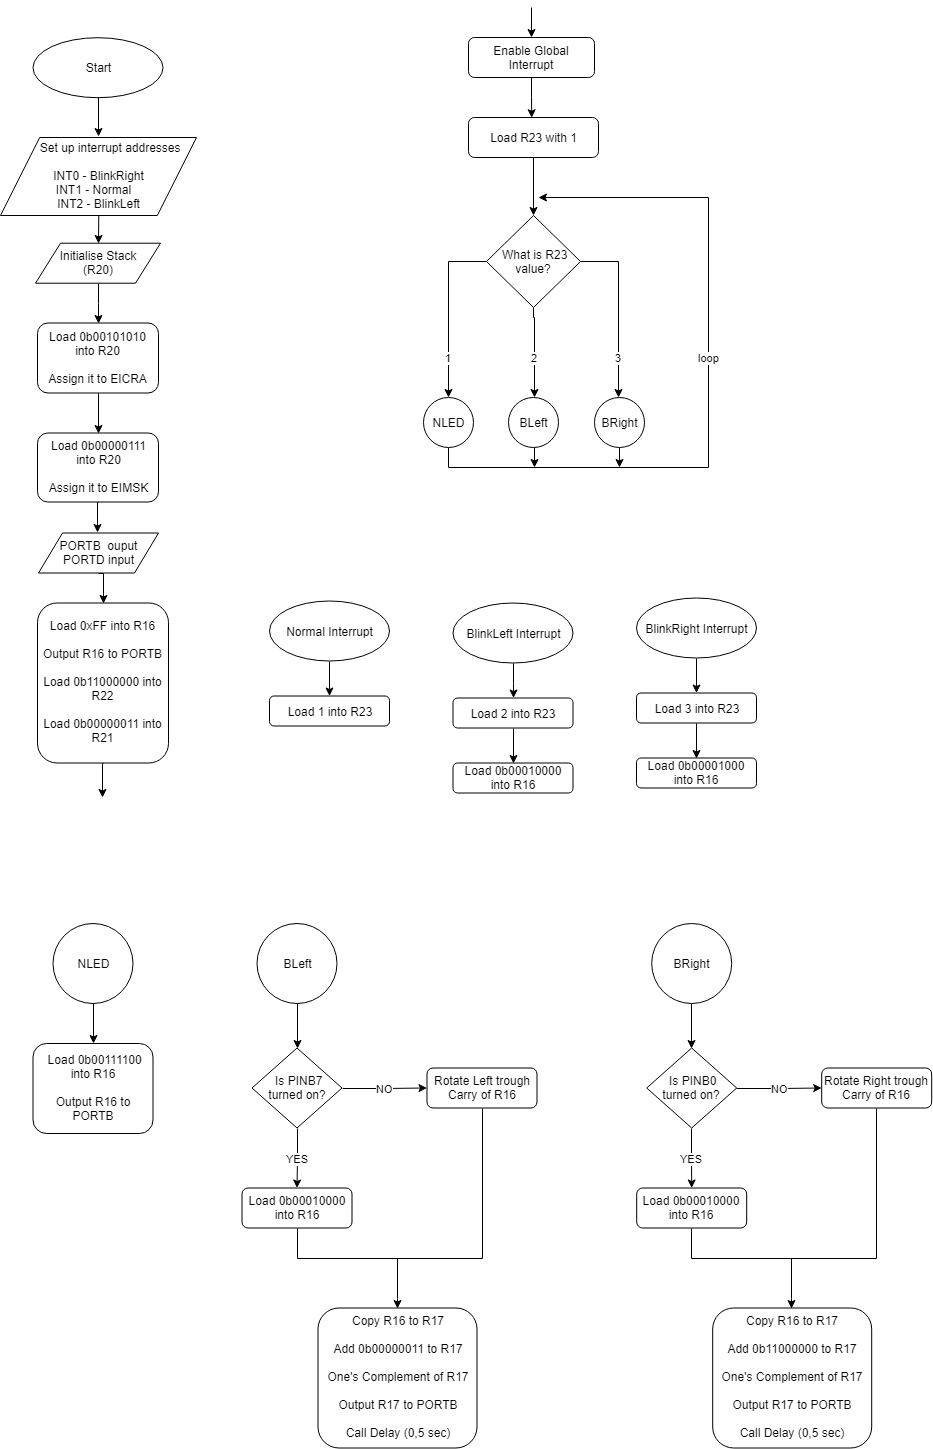
\includegraphics[scale=0.8]{img/TASK3.png}
\end{center}

\newpage
\section{Task 4 - Rear lights on a car, with light for brakes}

\lstset{style=Asm}
\begin{lstlisting}
;>>>>>>>>>>>>>>>>>>>>>>>>>>>>>>>>>>>>>>>>>>>>>>>>>>>>>>>>>>>
; 1DT301, Computer Technology I
; Date: 2019-09-29
; Author:
; Loic GALLAND
; Leonardo PEDRO
;
; Lab number: 3
; Title: How to use interrupts
;
; Hardware: STK600, CPU ATmega2560
;
; Function: Same program as Task 3, but now there is another Interrupt to simulate the brakes. When breaking all the lights needs to be turned on.
;			When blinking right LED7-4 light up and LED3-0 do Ring Counter to the right.
;			When blinking left LED3-0 light up & LED7-4 do Ring Counter to the left.
; Input ports: PORTD
;
; Output ports: PORTB
;
; Subroutines: If applicable.
; Included files: m2560def.inc
;<<<<<<<<<<<<<<<<<<<<<<<<<<<<<<<<<<<<<<<<<<<<<<<<<<<<<<<<<<<
.include "m2560def.inc"

.org 0x00
rjmp start

.org INT0addr	;Address of Interrupt 0, used for blinking right.
rjmp BlinkRight	

.org INT1addr	;Address of Interrupt 1, used for normal lights.
rjmp Normal_Interrupt

.org INT2addr	;Address of Interrupt 2, used for the break lights.
rjmp Press_Break

.org INT3addr	;Address of Interrupt 3, used for blinking left.
rjmp BlinkLeft

.org 0x72

start:
; Initialize SP, Stack Pointer
ldi r20, HIGH(RAMEND) ; R20 = high part of RAMEND address
out SPH,R20 ; SPH = high part of RAMEND address
ldi R20, low(RAMEND) ; R20 = low part of RAMEND address
out SPL,R20 ; SPL = low part of RAMEND address

ldi r20,0b10101010 ;Setting INT0-INT1-INT2-INT3 into falling edge
sts EICRA,r20
ldi r20,0b00001111 ;Enable INT0-INT1-INT2-INT3
out EIMSK,r20

ldi r17,0xFF	;Set PORTB as output
out DDRB, r17

ldi r17,0x00	;Set PORTD as input
out DDRD,r17

ldi r16, 0xFF	;Iniatialize the LEDs
out PORTB, r16

.def LED = r16	;Give the name "LED" to the register number 16
.def Normal_Right = r22	;Give the name "Normal_Right" to the register number 22, will be used to simulate the left rear light
ldi Normal_Right, 0b11000000
.def Normal_Left = r21	;Give the name "Normal_Left" to the register number 21 will be used to simulate the right rear light
ldi Normal_Left,0b00000011

sei	;Global interrupt enable


ldi r23, 1	;Variable to know in which configuration we are in.


Main:
	cpi r23,1	;If r23 = 1 then branch to NLED which is the normal LEDs:
	breq NLED

	cpi r23, 2	;If r23 = 2 then branch to BLeft which is the blinking to right.
	breq BRight

	cpi r23, 3	;If r23 = 3 then branch to BLeft which is the blinking to left.
	breq BLeft
rjmp Main

NLED:
	ldi LED, 0b00000000	;Load 0x00 into "LED", to "reset" it
	ADD LED,Normal_Right	;Add both side of the rear lights with binary code
	add LED,Normal_Left		; 0b11000011
	mov r17,LED	;Copy the info from LED
	COM r17	;One's complement of r17
	out PORTB, r17
rjmp Main

BLeft: ;RING COUNTER
	SBIS PORTB,PINB7 ;If the LED7 is on then reset the LEDs otherwise skip the next line
		ldi LED,0b00010000
	SBIC PORTB,PINB7	;If the LED7 is not on then Rotate otherwise skip the next line 
		rol LED;Rotate to the left 
	call Out_LED_Left	;call the method that will ouput to the LEDs
	call Delay	;Delay of 0.5 sec
rjmp main


BRight:
	SBIS PORTB,PINB0 ;If the LED0 is on then reset the LEDs otherwise skip the next line
		ldi LED,0b00001000
	SBIC PORTB,PINB0	;If the LED0 is not on then Rotate otherwise skip the next line 
		ror LED	;Rotate to the left 
	call Out_LED_Right	;call the method that will ouput to the LEDs
	call Delay	;Delay of 0.5 sec
rjmp main

Out_LED_Right:	;To output to PORTB the LEDs when it is going to the right
	mov r17,LED	;Copy the info from "LED" to r17
	add r17,Normal_Right	;Add "Normal_Right" to r17
	com r17	;One's Complement of r17. to switch the 0s into 1s 
	out PORTB,r17
RET	;Return to where the routine was called
Out_LED_Left:	;To output to PORTB the LEDs when it is going to the left
	mov r17,LED	;Copy the info from "LED" to r17
	add r17,Normal_Left	;Add "Normal_Left" to r17
	com r17	;One's Complement of r17. to switch the 0s into 1s 
	out PORTB,r17
RET	;Return to where the routine was called

Normal_Interrupt:	;Interrupt for the normal lights
ldi r23,1	;Load 1 into r23 to know later on in which program we are.
ldi Normal_Right, 0b11000000	;Load the correct binary code to Normal Right
ldi Normal_Left,0b00000011	;Load the correct binary code to Normal Left
RETI	;Return to where the interrupt "interrupted"

BlinkRight:	;Interrupt to when it's blinking right
ldi r23, 2	;Load 2 into r23 to know later on in which program we are.
ldi LED,0b00001000	;Initialise the LEDs
ldi Normal_Right, 0b11000000
ldi Normal_Left,0b00000011
RETI	;Return to where the interrupt "interrupted"

BlinkLeft:	;Interrupt to when it's blinking left
ldi r23, 3	;Load 3 into r23 to know later on in which program we are.
ldi LED,0b00010000
ldi Normal_Right, 0b11000000
ldi Normal_Left,0b00000011
RETI	;Return to where the interrupt "interrupted"
	
Press_Break:	;Interrupt for when we are breaking
	ldi Normal_Left,0b00001111
	ldi Normal_Right,0b11110000
RETI	;Return to where the interrupt "interrupted"
		


Delay:
; Generated by delay loop calculator
; at http://www.bretmulvey.com/avrdelay.html
; Delay 500 000 cycles
; 500ms at 1 MHz
    ldi  r18, 3
    ldi  r19, 138
    ldi  r20, 86
L1: dec  r20
    brne L1
    dec  r19
    brne L1
    dec  r18
    brne L1
    rjmp PC+1
RET
\end{lstlisting}

\newpage
This is the flowchart of the task 4:
\begin{center}
%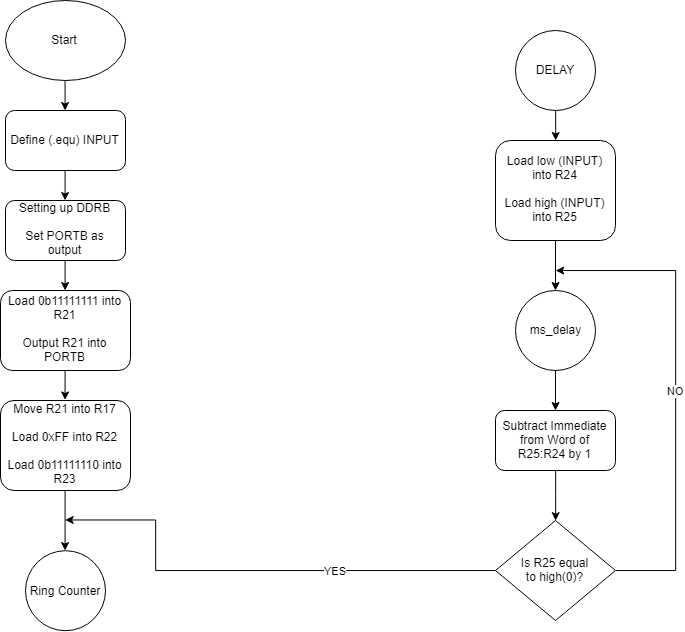
\includegraphics[scale=0.7]{img/Task4.png}
\end{center}
% Prints your bibliography database xxx.bib
\bibliographystyle{IEEEtran}
\bibliography{ref.bib}

\end{document}
